{\centering \nonumsubsection{B \hspace{1em} 组}}
\begin{xiaotis}
\setcounter{cntxiaoti}{26}

\xiaoti{设直线 $l_1$ 及 $l_2$ 在同一个平面内,$A = \{P | \text{点} P \in l_1 \}$,
    $B = \{Q | \text{点} Q \in l_2 \}$,问:}
\begin{xiaoxiaotis}
    
    \xiaoxiaoti{$A \cap B = \kongji$ 时,直线 $l_1$,$l_2$ 有什么关系。}

    \xiaoxiaoti{$A \cap B$ 是单元素集时,直线 $l_1$,$l_2$ 有什么关系。}

    \xiaoxiaoti{$A \cap B$ 含有两个以上元素时,直线 $l_1$,$l_2$ 有什么关系。}

\end{xiaoxiaotis}

\xiaoti{设集合 $I$,$A$,$B$,$C$ 的关系如图所示,并记 $\buji{A}$,$\buji{B}$,$\buji{C}$
    为 $A$,$B$,$C$ 在 $I$ 中的补集,用阴影表示下列集合:}
\begin{xiaoxiaotis}

    \begin{tabular}[t]{*{2}{@{}p{16em}}}
        \xiaoxiaoti{$\buji{A} \cap \buji{C}$;} &  \xiaoxiaoti{$(A \cap B) \cup C$;} \\
        \xiaoxiaoti{$\buji{(A \cap B)} \cap C$;} &  \xiaoxiaoti{$(A \cap B) \cup B$;} \\
        \xiaoxiaoti{$\buji{B} \cup C$;} & \xiaoxiaoti{$\buji{\buji{A} \cup \buji{B}}$。}
    \end{tabular}

\end{xiaoxiaotis}

\begin{figure}[htbp]
    \centering
    \begin{minipage}{8cm}
    \centering
    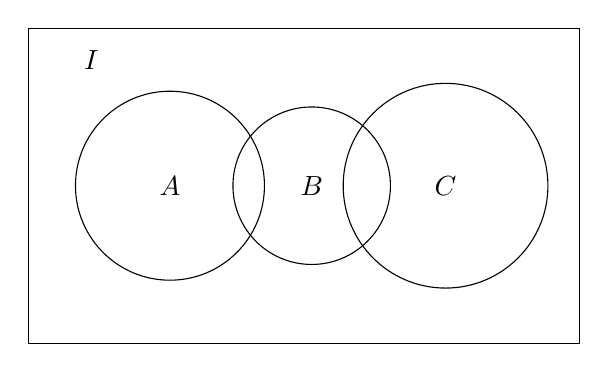
\begin{tikzpicture}
    \draw (0,0) circle (1.2) node{$A$};
    \draw (1.8,0) circle (1.0) node{$B$};
    \draw (3.5,0) circle (1.3) node{$C$};
    \draw (-1.8, -2) rectangle (5.2,2);
    \node at (-1,1.6) {$I$};
\end{tikzpicture}

    \caption*{(第28题)}
    \end{minipage}
    \qquad
    \begin{minipage}{8cm}
    \centering
    \begin{tikzpicture}[>=Stealth]
    \draw (0,0) rectangle (3,4);
    \filldraw[pattern=horizontal lines light gray] (0,0) rectangle (3,2);

    \draw (0,0) -- (0,-0.5) (3,0) -- (3,-0.5) [<->] (0,-0.35) -- (3,-0.35);
    \node [fill=white] at (1.5,-0.35) {$d$};
    
    \draw (0,0) -- (-0.5,0) (0,4) -- (-0.5,4) [<->] (-0.35,0) -- (-0.35,4);
    \node [fill=white] at (-0.35,2.5) {$h$};

    \draw (3,0) -- (3.5,0) (3,2) -- (3.5,2) [<->] (3.35,0) -- (3.35,2);
    \node [fill=white] at (3.35,1) {$x$};

    \draw (1.5,4.5) [rounded corners=.3cm] -- (1.5,5.5)-- (2.5,5.5);
    \draw (1.8,4.5) [rounded corners=.25cm] -- (1.8,5.2)-- (2.5,5.2);
    \draw[pattern=dots,pattern color=gray,dotted] (1.5,4.5) -- (1.8,4.5) -- (2.0,2) -- (1.2,2) -- cycle;
\end{tikzpicture}

    \caption*{(第29题)}
    \end{minipage}
\end{figure}

\xiaoti{如图,一个圆柱形容器的底部直径是 $d$ 厘米,高是 $h$ 厘米。现在以每秒钟 $s \,\text{厘米}^3$
    的速度向容器内注入某种溶液。求容器内溶液的高度 $x$ 与注入溶液的时间 $t$ 之间的函数关系式。
    并写出函数的定义域与值域。}

\xiaoti{某人开汽车以 $60$ 公里/小时的速度从 $A$ 地到 $150$ 公里远处的 $B$ 地,在 $B$ 地停留 $1$
    小时后,再以 $50$ 公里/小时的速返回 $A$ 地。把汽车离开 $A$ 地的路程 $x$ 公里表示为时间 $t$
    小时(从 $A$ 地出发时开始)的函数,并画出函数的图象;又把车速 $v$ 公里/小时表示为时间 $t$
    的函数,并画出函数的图象}

\xiaoti{设 $f(x) = x^2$,$g(x) = 2x -5$,比较 $f(g(x))$ 和 $g(f(x))$ 是否一样。}

\xiaoti{已知 $f(x) = (x^2 + 2)^2 - 4(x^2 + 2) + 4$,求证}
$$f(tx) = t^4 f(x) \text{。}$$

\xiaoti{}
\begin{xiaoxiaotis}

    \vspace{-0.9em}
    \begin{minipage}{0.94\textwidth}
        \xiaoxiaoti{已知奇函数 $f(x)$ 在区间 $[a, b]$ 上 $(0 < a < b)$ 是减函数,那么它在区间 $[—b,-a]$ 上是增函数还是减函数?}

    \end{minipage}
    \vspace{0.5em}

    \xiaoxiaoti{已知偶函数 $g(x)$ 在区间 $[a, b]$ 上 $(0 < a < b)$ 是减函数,那么它在区间 $[—b,-a]$ 上是增函数还是减函数?}

\end{xiaoxiaotis}

\xiaoti{设 $f(x)$ 是定义在 $R$ 上的任一函数,求证 $F_1 (x) = f(x) + f(-x)$ 是偶函数,$F_2 (x) = f(x) - f(-x)$ 是奇函数。}

\xiaoti{设在离海平面高度 $x$ 米处的大气压强是 $y$ 毫米水银柱高,$y$ 与 $x$ 之间的函数关系式是
    $$y = Ce^{kx} \text{,}$$
    这里 $C$,$k$ 都是常量。已知某地某天在海平面及 $1000$ 米高空的大气压强分别是 $760$ 及 $675$
    毫米水银柱高,求在 $600$ 米高空的大气压强,又求大气压强是 $720$ 毫米水银柱高处的高度(结果都保留三位有效数字)。}
    
\xiaoti{把物体放在冷空气中冷却,如果物体原来的温度是 $\theta_1$ 度,空气的温度是 $\theta_0$ 度,
    $t$ 分钟后物体的温度 $\theta$ 度可由公式
    $$\theta = \theta_0 + (\theta_1 - \theta_0)e^{-kt}$$
    求得,这里 $k$ 是一个随着物体与空气的接触状况而定的正的常量。现有 $62^\circ C$ 的物体,放在
    $15^\circ C$ 的空气中冷却,$1$ 分钟以后物体的温度是 $52^\circ C$,求上式中的 $k$ 值,然后
    计算开始冷却后多少分钟物体的温是 $42^\circ C$,$32^\circ C$,$22^\circ C$,$15.1^\circ C$
    (精确到一个有效数字)。物体会不会冷却到 $12^\circ C$?}

\xiaoti{求下列函数的定义域、值域:}
\begin{xiaoxiaotis}

    \begin{tabular}[t]{*{2}{@{}p{16em}}}
        \xiaoxiaoti{$y = \dfrac{x + 1}{x + 2}$;} &  \xiaoxiaoti{$y = -\sqrt{x^2 + 25}$;} \\
        \xiaoxiaoti{$y = \dfrac{1}{(x - 1)(2x - 1)}$;} &  \xiaoxiaoti{$y = x + \sqrt{1 - 2x}$。}
    \end{tabular}
    \vspace{0.5em}

\end{xiaoxiaotis}

\xiaoti{}
\begin{xiaoxiaotis}

    \vspace{-1.7em}
    \begin{minipage}{0.94\textwidth}
        \xiaoxiaoti{已知 $\ln y = x + \ln C$,求证 $y = Ce^x$;}

    \end{minipage}

    \vspace{0.5em}
    \xiaoxiaoti{已知 $ln \dfrac y x - ax = \ln C$,求证 $y = Cxe^{ax}$。}
    \vspace{0.5em}

\end{xiaoxiaotis}

\xiaoti{设 $a^2 + b^2 = 7ab$,且 $a > 0$,$b > 0$,求证}
$$\lg \dfrac{a + b}{3} = \dfrac 1 2 (\lg a + \lg b) \text{。}$$

\xiaoti{求下列函数的定义域:}
\begin{xiaoxiaotis}
    
    \twoInLine[16em]{\xiaoxiaoti{$y = \sqrt{3^x -9}$;}}{\xiaoxiaoti{$y = \sqrt{1 - a^x} \, (0 < a < 1)$;}}

    \xiaoxiaoti{$y = \log_a (6x^2 - x - 2) \, (a > 0 \text{,且} a \neq 1)$;}

    \xiaoxiaoti{$y = \log_a (-x^2 + 4x -3) \, (a > 0 \text{,且} a \neq 1)$。}

\end{xiaoxiaotis}

\xiaoti{}
\begin{xiaoxiaotis}

    \vspace{-1.7em}
    \begin{minipage}{0.94\textwidth}
        \xiaoxiaoti{方程 $3^{2x^2} = 3^{5x + 7}$ 与方程 $2x^2 = 5x + 7$ 的解集是否相等,为什么?}

    \end{minipage}

    \xiaoxiaoti{方程 $\log_2 2x^2 = \log_2 (x + 6)$ 与方程 $2x^2 = x + 6$ 的解集是否相等,为什么?}

    \xiaoxiaoti{方程 $\lg (x - 1) + \lg (x - 2) = \lg (x + 2)$ 与方程 $(x - 1) \cdot (x - 2) = x + 2$ 的解集是否相等,为什么?}

\end{xiaoxiaotis}

\xiaoti{解下列方程组:}
\begin{xiaoxiaotis}
    
    \begin{tabular}[t]{*{2}{@{}p{16em}}}
        \xiaoxiaoti{$
            \begin{cases}
                9^{x + y} = 729, \\
                3^{x - y - 1} = 1 ;
            \end{cases}
        $} &  \xiaoxiaoti{$
            \begin{cases}
                2^x \cdot 3^y = 648, \\
                3^x \cdot 2^y = 432;
            \end{cases}
        $} \\
        \xiaoxiaoti{$
            \begin{cases}
                \lg x + \lg y = 5, \\
                \lg x - \lg y = 3 ;
            \end{cases}
        $} &  \xiaoxiaoti{$
            \begin{cases}
                x - y = 90, \\
                \lg x + \lg y = 3 \text{。}
            \end{cases}
        $}
    \end{tabular}

\end{xiaoxiaotis}

\end{xiaotis}
